\documentclass{book}
\usepackage[utf8]{inputenc}

%
%	landscape orientation 
%
\usepackage[ngerman]{babel}
\usepackage[landscape]{geometry}
\usepackage{times}
\usepackage{multicol}
\usepackage{graphicx}
\usepackage{geometry}
\usepackage{lipsum}
\usepackage{verbatim}
\usepackage{eso-pic}
\usepackage{fancyhdr}
\usepackage{tikz}
\usepackage{titlesec}
\usepackage{pdfpages}

% \titleformat{\chapter}[display]
%   {\normalfont\bfseries}{}{0pt}{\Huge}
% \titleformat{\section}[display]
%   {\normalfont\bfseries}{}{0pt}{\Large}
%   \titleformat{\subsection}[display]
%   {\normalfont\bfseries}{}{0pt}{\Large}

\titleformat{\chapter}{\normalfont\huge\bfseries}{}{0em}{}
\titleformat{\section}{\normalfont\Large\bfseries}{}{0em}{}
\titleformat{\subsection}{\normalfont\large\bfseries}{}{0em}{}
\titleformat{\subsubsection}{\normalfont\normalsize\bfseries}{}{0em}{}
\titleformat{\paragraph}[runin]{\normalfont\normalsize\bfseries}{}{0em}{}
\titleformat{\subparagraph}[runin]{\normalfont\normalsize\bfseries}{0}{0em}{}

\fancypagestyle{plain}{
    \lhead{}
	\fancyhead{}
    \fancyfoot{}
    \renewcommand{\headrulewidth}{0pt}
}

\pagestyle{fancy}
\fancyhead[R]{\leftmark{}}
\fancyhead[L]{}
\renewcommand{\headrulewidth}{0pt}
\renewcommand{\chaptermark}[1]{\markboth{#1}{}}
\fancyfoot{}
\fancyfoot[R]{\thepage}

\renewcommand{\chaptermark}[1]{\markboth{#1}{}}
\renewcommand{\subsectionmark}[1]{\markboth{#1}{}}

\begin{document}

%\input{./chap/cover.tex}

%HERE YOU CAN CHANGE THE MARGIN SIZE
\newgeometry{left=2cm,right=2cm,outer=2cm,inner=2cm}
%DISTANCE BETWEEN COLUMNS 
\setlength\columnsep{30pt}


\chapter{Die ersten Jahre}
\input{./chap/Gründung.tex}
% \begin{figure}[p]
% 	\centering
% 	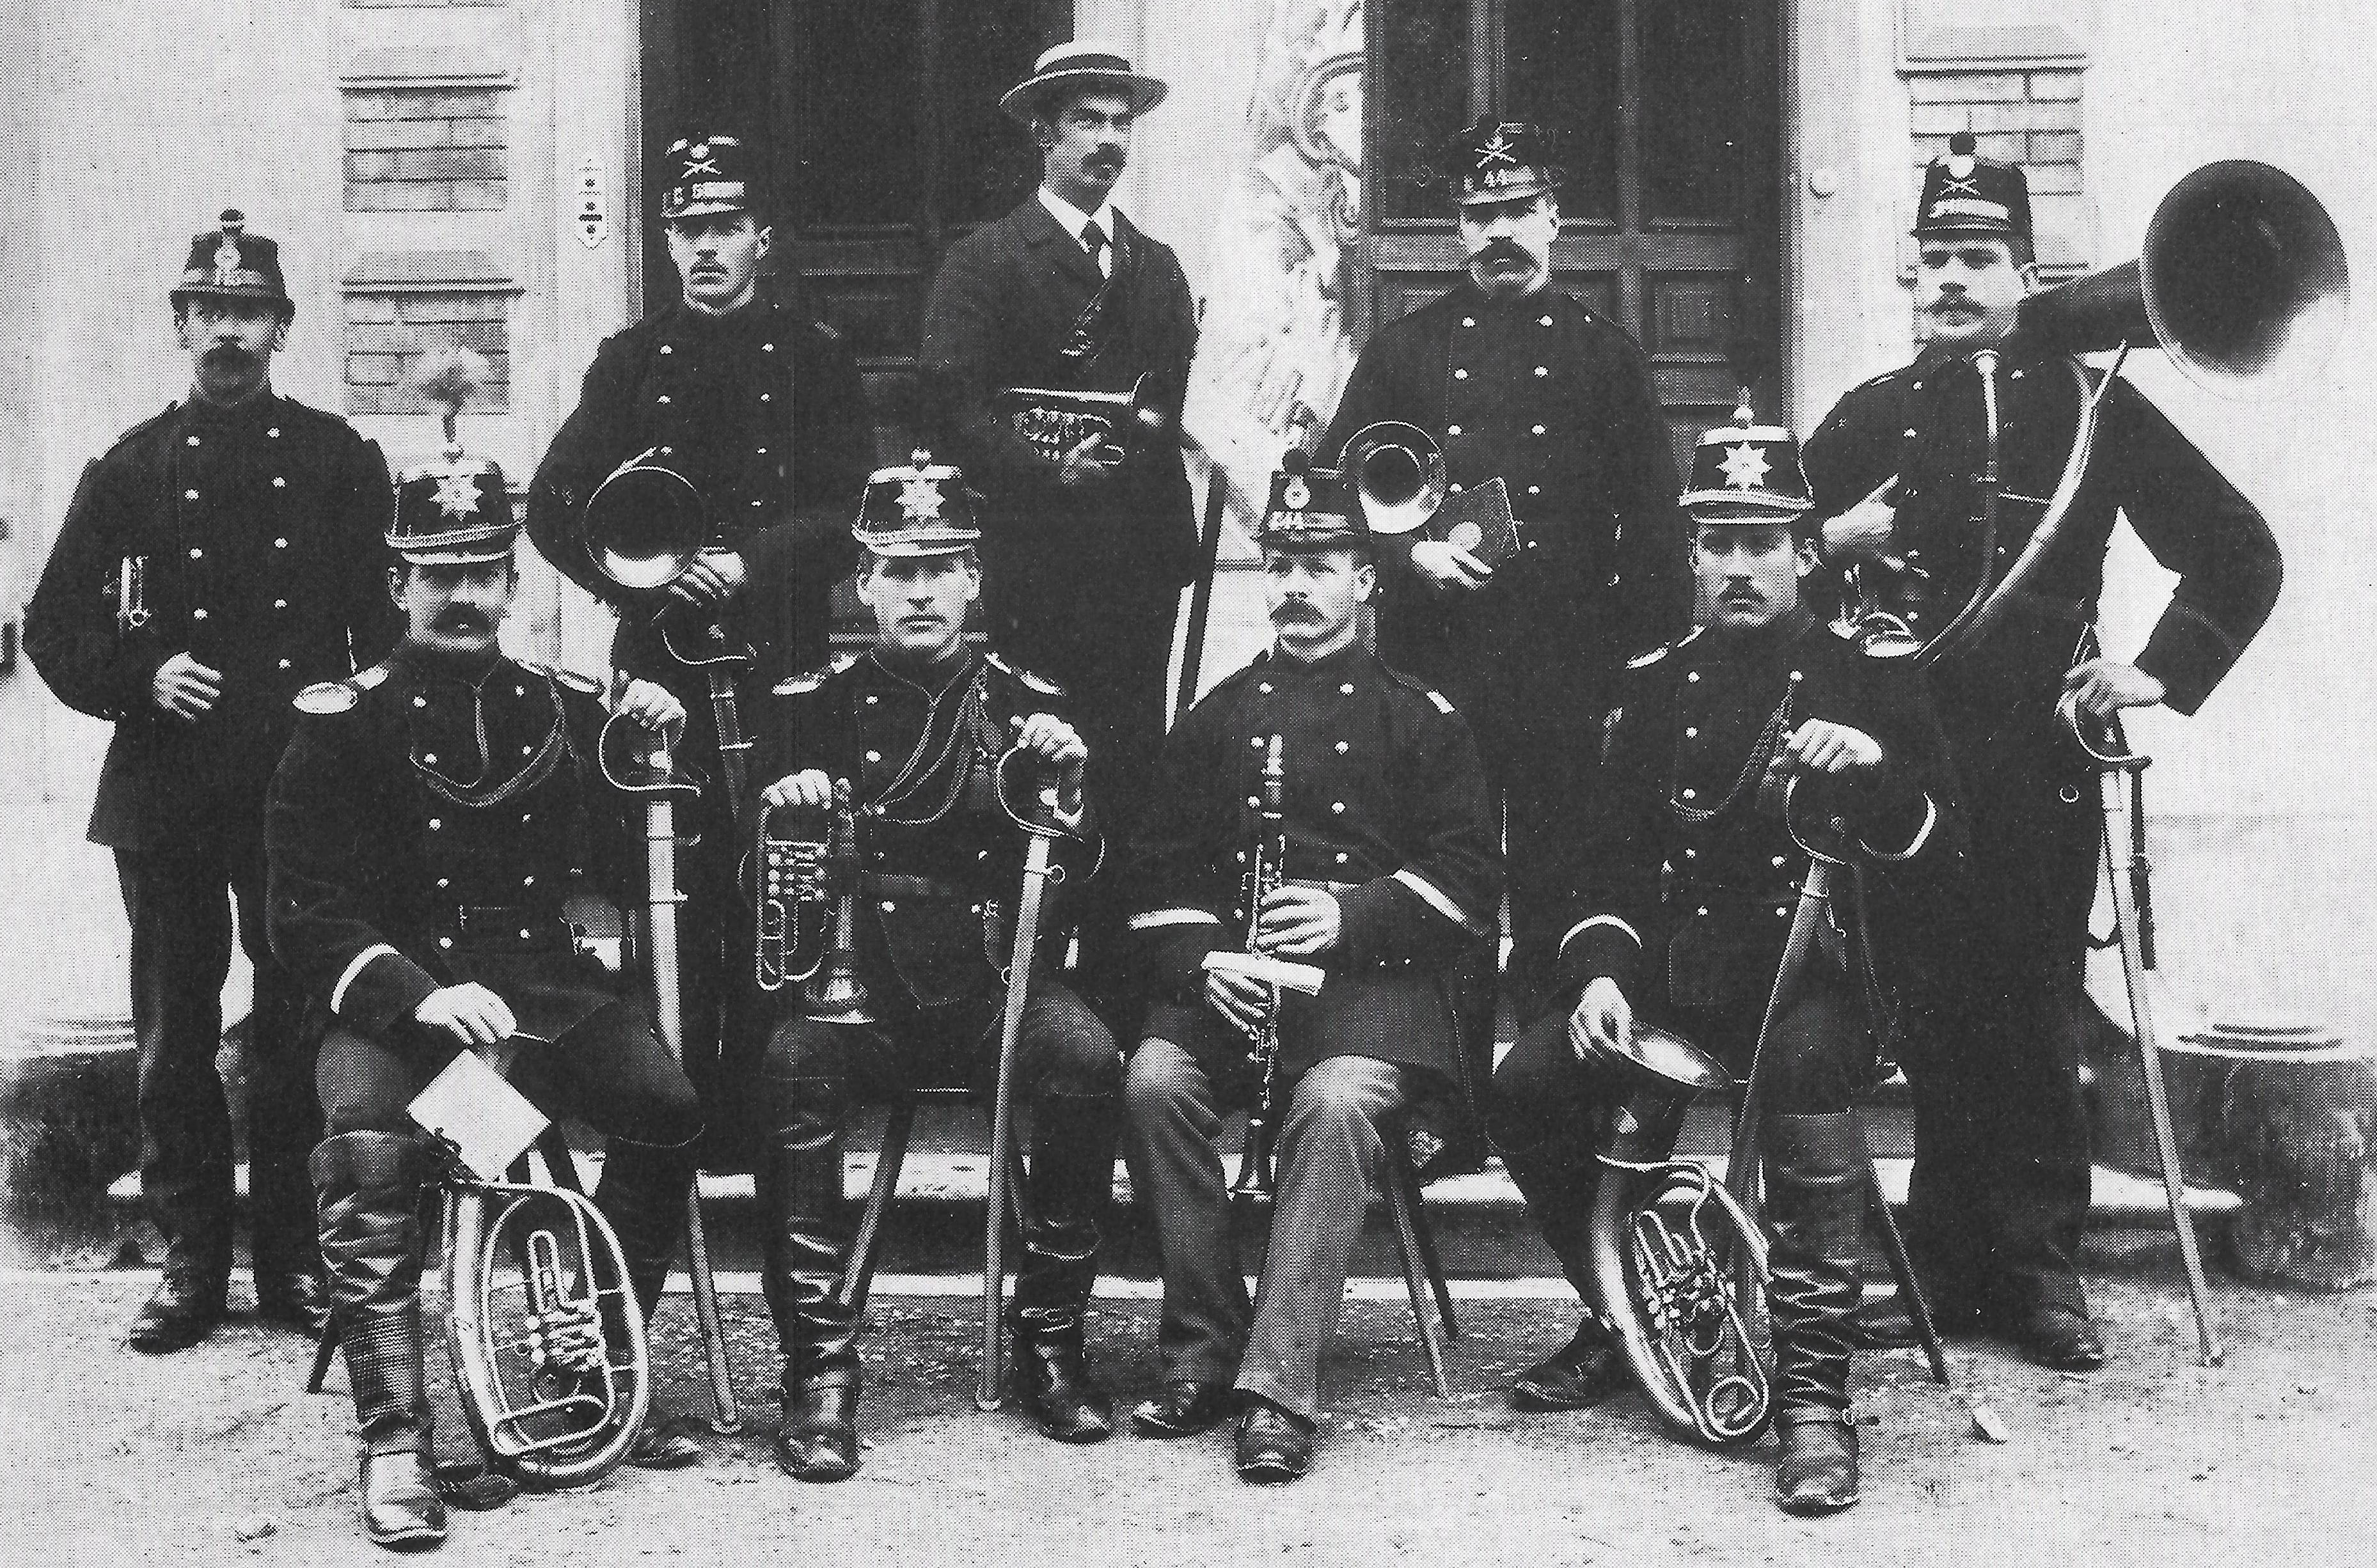
\includegraphics{./chap/MGH-1905.jpg}
% 	\caption{1905}
% 	\label{fig:meine-grafik}
% \end{figure}
% \pagebreak

\begin{multicols}{2}

    \subsection{Statuten vom 25. März 1876}

    Es hat sich in der Gemeinde Hildisrieden unter obigem
    Datum eine neue Musikgesellschaft gebildet, welche
    den Mitgliedern zum besseren Gedeihen der Gesellschaft
    folgende Bedingungen festgesetzt:

    \S1
    Jedes Mitglied soll, wenn möglich, lange bei der Gesellschaft
    verbleiben und dieselbe fördern.

    \S2
    Die Gesellschaft bildet sich nicht nur zum Schein, sie
    will auch etwas erlernen, um sich auch produzieren zu
    können, daher verpflichtet sich jedes Mitglied, an den
    vorhergesagten Proben zu erscheinen.

    \S3
    Zum Bestimmen der Proben, sowie zum Dirigieren
    wählt die Gesellschaft einen Kapellmeister.

    \S4
    Wer an der Probe 20 Minuten zu spät erscheint, der
    wird um 20 Cts., wer eine halbe Stunde zu spät kommt
    um 30, und wer gar nicht erscheint, um 50 Cts. bestraft.

    \S5
    Wenn es gewisse Umstände verlangen, so ist der Kapellmeister
    berechtigt, festzustellen, was von den Mitgliedern bis zur
    nächsten Probe gelernt werden soll.

    \S6
    Wird etwas nicht gelernt und man sieht, dass es flissentlich
    nicht geschehen ist, so ist der Betreffende in
    eine Strafe von 30 Cts. verfallen, die jedoch auch erhöht werden
    kann bis auf einen Franken.

    \S7
    Kann sich ein Mitglied mit der Gesellschaft nicht mehr
    vertragen, so steht es dieser frei, das Mitglied auszuschliessen,

    \S8
    Tritt ein Mitglied nach eigener Willkür aus der Gesellschaft,
    so hat es eine Entschädigung von 20 Fr. zu entrichten.

    \S9
    Wer nicht mehr an den Proben erscheint, der schliesst
    sich von selbst aus der Gesellschaft und die Entschädigung folgt.
    Die Gelder, Strafgelder sowie andere, sind vom Präsidenten einzuziehen
    und er hat die Pflicht, zu besorgen und am Ende des Jahres oder wenn
    es die Gesellschaft verlangt, genaue Rechnung abzugeben.

    \S10 |
    Was Instrumente anbetrifft, so hat jedes Mitglied das
    seinige selbst anzuschaffen und zu besorgen. Ein
    schlechtes Instrument wird nicht geduldet.

    \S12
    Wenn 2/3 der Mitglieder einen Ausmarsch verlangen,
    und ein Mitglied will oder kann nicht kommen, so hat
    es dieser sofort dem Kapellmeister anzuzeigen, sonst
    ist es in eine Strafe von drei Fr. verfallen. Die Gesellschaft
    zieht dann eine andere Person zu und das betreffende Mitglied
    hat selbe zu entschädigen und ihr sein Instrument zu leihen.

    \S13
    Jedes Mitglied soll sich dem Befehl des Kapellmeisters
    und Präsidenten fügen soweit ihnen die Gesellschaft
    das Recht in die Hand gelegt hat.

    \S14
    Kommt etwas vor, das in dem Rechte dieser zwei Personen liegt,
    so wird die Gesellschaft angefragt, und es wird abgestimmt.

    \S15
    Tritt ein neues Mitglied in die Gesellschaft, so hat es eine
    Eintrittszahlung von zehn Fr. zu entrichten und sein Instrument
    anzuschaffen. Dann tritt es in die gleichen Rechte wie die andern Mitglieder.

    \S16
    Auch diese, so wie alle andern Gelder werden vom Präsidenten
    bezogen und er hat am Ende des Jahres genaue Rechnung abzugeben,
    wonach die Gelder unter die Mitglieder gleichmässig verteilt werden.
    Am Ende Jahres hat jedoch ein Saldo von 20 Fr. in der Kasse
    zu bleiben, das zum Anschaffen neuer Musikstücke
    aufs folgende Jahr verwendet wird.

    \S17
    Die Musikstücke werden vom Präsidenten oder Kapellmeister bestellt, sie
    haben jedoch die Gesellschaft zuerst anzufragen.

    \S18
    Die bestellten Stücke werden vom Präsidenten bezahlt
    und er hat darüber Rechnung zu geben.

    \S19
    Würde es der Fall sein, dass ein Mitglied stürbe, so
    würde die Gesellschaft für dasselbe einen angemessenen
    Gottesdienst halten lassen,

    \S20
    Wer bei der Musik sein will, muss auch in die Gesellschaft treten.

    \S21
    Die Gesellschaft wählt einen Vorstand von 3 Mit-
    gliedern: Kapellmeister, Präsident und Schreiber auf
    eine Amtsdauer von zwei Jahren.

    \S22
    Der Schreiber schreibt die Stücke und alles, was die
    Gesellschaft beschlägt, wofür er angemessen entschädigt
    wird.

    \S23
    Als Entschuldigung wird in allen Fällen nur Krankheit oder Militärdienst angenommen.

    \S24
    Jedes Mitglied hat sich eigenhändig zu unterzeichnen.\\


\end{multicols}

% \begin{figure}[p]
% 	\centering
% 	\includegraphics[scale=0.5]{./chap/MGH-Statuten-1874-S1.jpg}
% 	\caption{1905}
% 	\label{fig:Statuten-1874}
% \end{figure}
% \begin{figure}[p]
% 	\centering
% 	\includegraphics[scale=0.5]{./chap/MGH-Statuten-1874-S2.jpg}
% 	\caption{1905}
% 	\label{fig:Statuten-1874}
% \end{figure}
\begin{multicols}{2}

    \section{Die Musikgesellschaft Hildisrieden im Jahre 1874}

    1875 — 1900

    Die Wiegenjahre brachten der Musikgesellschaft Hildisrieden abwechslungsreiche Begebenheiten.

    Die Hauptbetätigung blieb weiterhin das Konzertieren in Form von Ständchen und Ausmärschen,
    in- und ausserhalb der Gemeinde, So treffen wir die Musikgesellschaft
    1882 im Emmenbaum anlässlich einer Theateraufführung und 1887 beritten am Auffahrtsumritt in Sempach. Die Entschädigung,
    welche die Musikgesellschaft von der Kirchenverwaltung Sempach erhielt, betrug immerhin 45 Franken. Ein Gesuch, den
    Auffahrtsumritt abwechslungsweise mit der Musikgesellschaft Sempach alle drei Jahre bestreiten zu dürfen, wurde von der Kirchenverwaltung abgelehnt.
    Was unseren Musikanten in den 1890er Jahren vorgeworfen werden konnte,
    war der Mangel an Ordnung    und Disziplin. Wohl hatte man 1884 neue Statuten
    aufgestellt und neue Strafbestimmungen festgesetzt; diese sind aber nicht
    von allen befolgt worden. Diese unruhigen Vereinsjahre, fünf an der Zahl,
    hatten zur Folge, dass man mit dem Gedanken spielte, die Musikgesellschaft
    aufzulösen oder sich den gegebenen Statuten zu fügen.

    Man fand sich hin und wieder zusammen und kam
    ebenso schnell wieder auseinander, bis schliesslich die
    Vernunft siegte. Ein weiterer Grund, der den Zusammenhang des
    Vereins trübte, war der kleine finanzielle Beitrag der Gemeinde.
    Jährlich 20 Franken waren wirklich kein grosses Honorar, wenn man bedenkt,
    dass jeder Musikant sein Instrument selbst zu beschaffen und
    die Musikgesellschaft an sämtlichen Prozessionen teilzunehmen hatte.

    Im Jahre 1899 wurde das Restaurant Kreuz eröffnet und der Saal
    im «Löwen» eingeweiht. Die Einladung zu diesen Festen fügte das
    schwache Gebilde wieder zusammen.

    Die Statuten von 1874 und 1884 erneuert, haben 10
    Mitglieder unterzeichnet. Es sind: Silvester Schnieper,
    Josef Wolf, Leonz Geisshüsler, Silvester Disler, Josef
    Disler, Peter Troxler, Peter Muff, Rudolf Bühlmann,
    Josef Wolf und Niklaus Süess.

    Weitere Einnahmen wurden mit dem «Umblasen»  während der Weihnachtszeit
    in der Gemeinde erzielt. Vor den Häusern wurde jeweils musiziert, wofür die
    Musik-freundlichen Bewohner eine Geldgabe spendeten.
    Im Jahre 1886 brachte der Verein auf diese Weise Fr. 259.60 zusammen.
    Bei kaltem Wetter war das Musizieren kein Vergnügen, denn öfters froren
    die Ventile ein und mussten durch Einhauchen wieder beweglich gemacht werden.
    Gerne wurde dann die Einladung angenommen, ins Haus zu kommen.

    In der warmen Stube liess es sich bequemer musizieren, besonders da,
    wo auch «Mittel» gegen trockene Kehlen bereitstanden.
    Allzulange aber durfte die Gastfreundschaft nicht beansprucht werden,
    warteten doch noch viele Einwohner auf den Besuch der Musikanten.
    War aber dann das gesteckte Tagesziel erreicht, wurde
    es mit dem Aufbruch nicht so genau genommen, gar
    wenn es oft etwas Feines zum Beissen gab.

    Leider ist nun auch dieser alte Brauch verschwunden.
    Dass es hin und wieder gemütlich wurde, berichtet
    die Chronik. Als beim Ausflug auf den Napf ein
    Leiterwagen mit Blumen und Girlanden geschmückt
    dem Sempachersee entlang rasselte, löste sich vom
    Wagen ein Rad, sodass ein Musikant nach dem andern
    vom Wagen kippte. Dabei gab es einige defekte
    Instrumente. Diese konnten in Willisau beim Instrumentenmacher Badmann wieder hergestellt werden.
    Die Fahrt führte ins Luthernbad und von da an zu
    Fuss auf den Napf. Dem Bassisten Troxler war das
    Bergsteigen nicht besonders angenehm, denn er soll sich
    damals geäussert haben: «Dass mer au uf ne so ne Morgelandssiech cha go!»



\end{multicols}


\pagebreak
\chapter{1974-1984}
\section{1974}
\begin{figure}[p]
    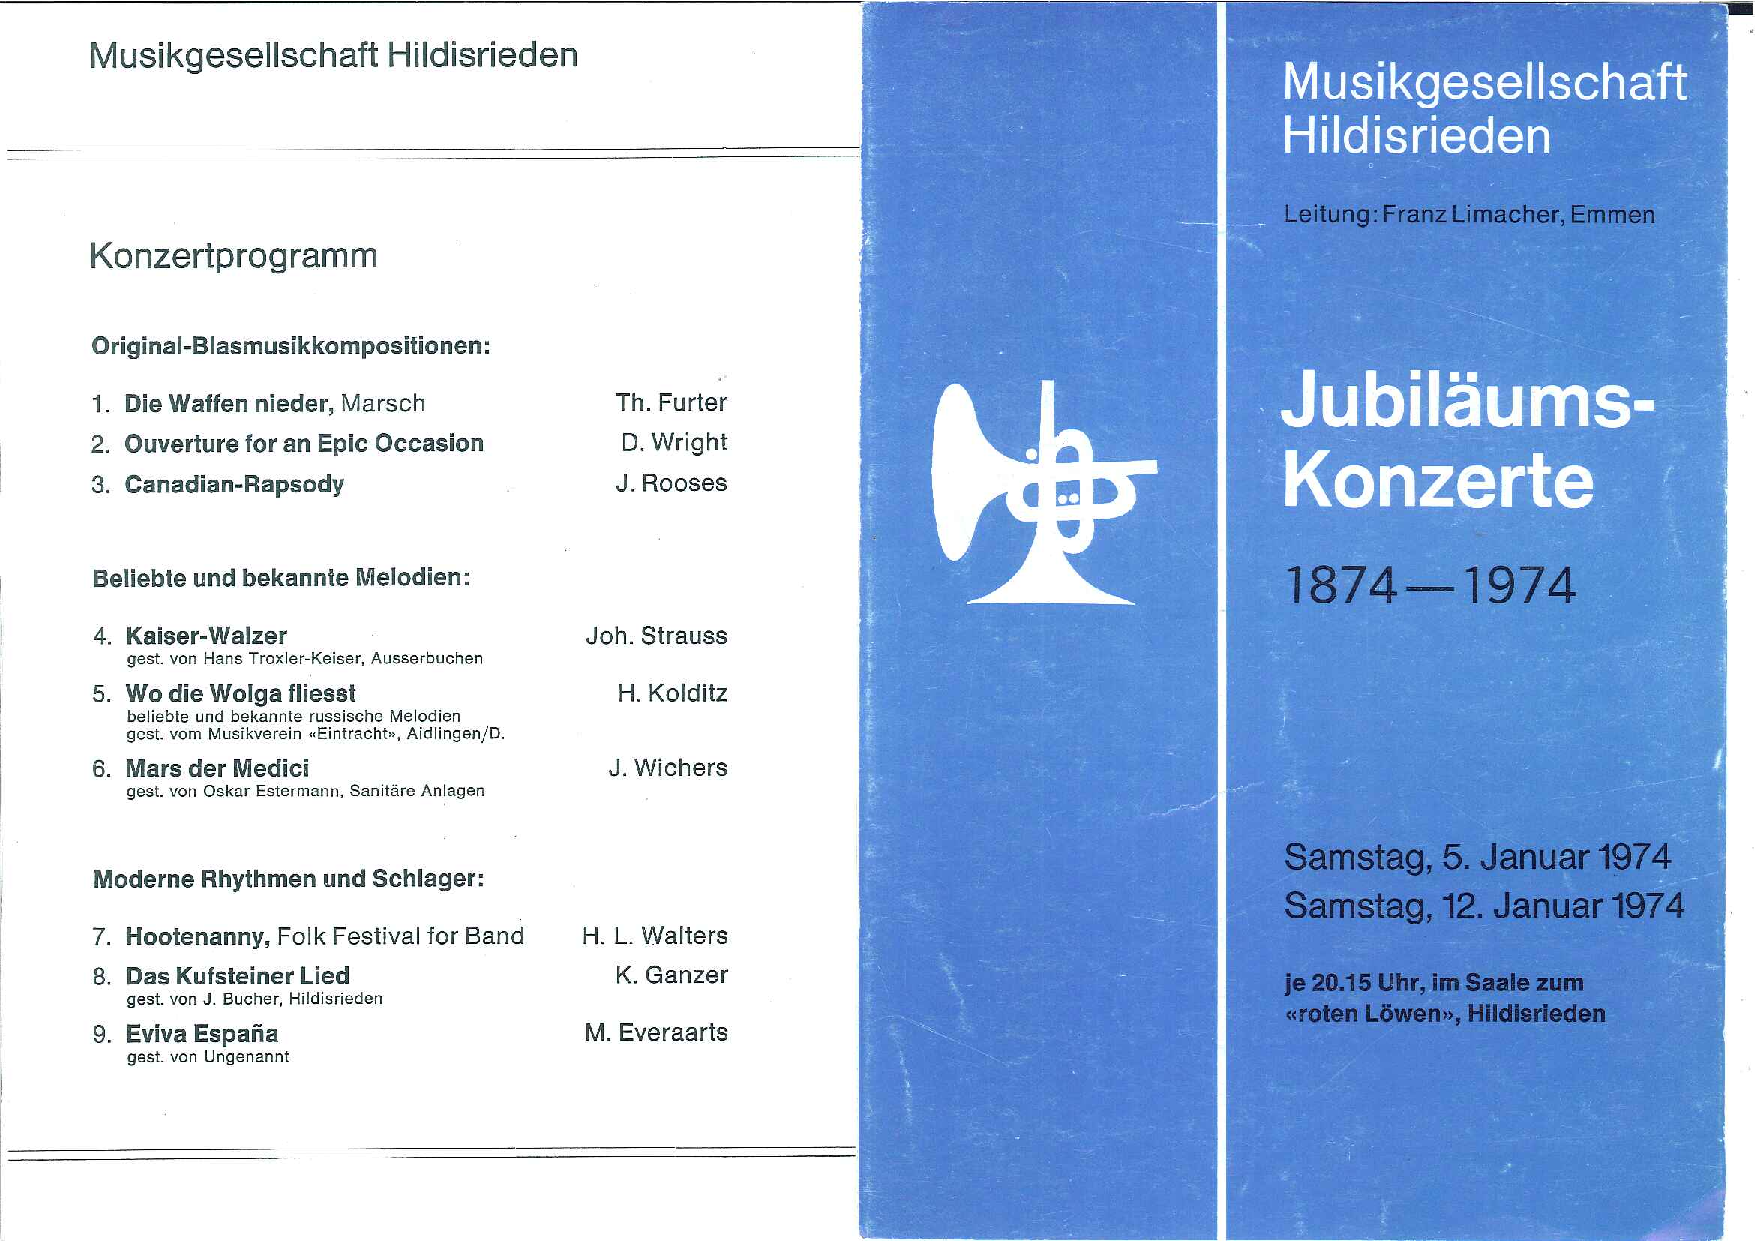
\includegraphics[scale=0.7]{./chap/1974/1974.pdf}
\end{figure}
\begin{multicols}{2}

    % \subsection{Jahresbericht}

    \begin{itemize}
        \item[]3. Jan.\\
        Bei der Probe macht der Präsident den Vorschlag
        des Vorstandes, beim Winterkonzert dem Verein aus finanziellen
        Gründen kein Nachtessen mehr zu bezahlen, dafür beim
        Konzert in Emmen ein Bier zu offerieren. Ohne
        Diskussion wird der Vorschlag angenommen.

        \item[]5. und 12. Jan.\\
        An diesen Abenden bringen wir das Jubiläumskonzert
        zu Gehör. Wir können uns an einem vollbesetzten
        Saal erfreuen. Eintritte 600 Personen. Seit mehreren Jahren
        konnten wir nicht mehr so viele Zuhörer begrüssen.

        \item[]10. Jan.\\
        Auch dieses Jahr pilgern wir nach Emmen um das
        Winterkonzert auch der Emmer Bevölkerung zu Gehör zu
        bringen. Der Reinerlös soll dieses Jahr an das seraphische
        Liebeswerk weitergeleitet werden. Aber es wird sich bloss um ein
        Trinkgeld handeln, denn die Zuhörerzahl beschränkt sich auf
        ca. 60 Stück. Nachher inkludieren wir im Restaurant
        Sternen noch ein Bier.

        \item[]18. Jan.\\
        Zunftbot im Rest. Kreuz. Um 1/4 vor 8 Uhr besammeln
        wir uns beim letztjährigen Zunftmeister Josef Estermann
        Bauernhof um noch unter seiner Macht den letzten Tropfen
        zu geniessen. Aber es soll noch nicht der letzte sein an diesem
        Abend, denn es regnet während des Einzuges ins Kreuz in Strömen.

        Der zum letzten mal amtierende Zunftpräsident
        Albin Estermann gibt die Nomination von Alois
        Gassmann Sandgütsch als neuer Zunftmeister bekannt.
        Mit grossem Applaus wird er in sein Amt eingesetzt.

        \item[]1. Feb.\\
        100. Generalversammlung im Rest. Kreuz

        \item[]2. Feb.\\
        Die Firma Schuler aus Rothenturm hat unsere Uniform im
        Rohbau soweit fertig, dass sie heute jedem Musikanten
        angepasst werden kann.

        \item[]15. Feb.\\
        Der Zunftmeister Alois Gassmann besucht die
        Schüler. Um 15 Uhr besammeln wir uns beim neuen
        Schulhaus. Dann gehts mit Marschmusik durchs Dorf
        zum alten Schulhausplatz. Dort bringen wir einige Stücke zu
        Gehör und der Zunftmeister lädt uns zu einem Imbiss
        im Kreuz ein.

        \item[]21. Feb.\\
        Da es schmutziger Donnerstag ist führen wir am
        Abend den traditionellen Musikhock im Kreuz durch.
        Es geht bald so richtig fastnächtlich zu. Es erscheinen gegen
        20 Maskierte, was für den kleinen Raum doch schon viel ist.
        Bei einer zügigen Tanzmusik, die Hugo Fleischlin organisiert
        hat, kommt Jung und Alt in den Genuss des Beinschwingens.

        \item[]5. März\\
        Herr Schuler jun. aus Rothenturm orientiert uns über sein
        Krawattensortiment. Mit grossem Mehr wird beschlossen,
        eine gemusterte Krawatte zur neuen Uniform zu kaufen.

        \item[]11. März\\
        OK Präsident Julius Bieri lädt den Verein ein zur Verteilung
        der Adressen für die Bettelaktion. Jedem
        anwesenden Musikanten werden einige Posten zugeteilt, sodass
        dem Kassier von heute an die Säcke bald gefüllt werden sollten.

        \item[]20. März\\
        Begrüssung der Neuzuzüger. Der Gemeinderat
        lädt alle 132 Neuzugezogenen in den Löwen ein. Auch
        unser Verein begrüsst sie auf musikalische Weise.

        \item[]2. April\\
        Firma Schuler aus Rothenturm liefert die neuen
        Uniformen an den Verein aus. Jeder Musikant
        kleidet sich ein. An 6 Hosen muss eine kleine Abänderung
        vorgenommen werden. Herr Schuler muntert uns
        auf zur neuen Uniform Sorge tu tragen, wenigstens
        die ersten paar Jahre.

        \item[]4. 5. 7. Mai \textbf{100-Jahr Feier der Musikgesellschaft Hildisrieden}\\
        Das Jubiläumsfest beginnt mit einem festlichen Eröffnungskonzert
        am Samstagabend, an dem die alte, stahlblaue Uniform
        mit rassigen Klängen verabschiedet wird. Der befreundete Musikverein Aidlingen aus
        Deutschland gibt ein Galakonzert in der zum Bersten gefüllten Festhalle
        und bringt auch  das Bierzelt mit Stimmungsmusik auf jubilierende Hochstimmung.

        Mit der Totenehrung auf dem Friedhof beginnt das sonntägliche Programm, und der
        Marsch "`alte Kameraden"' erklang in den Sonntagmorgen. Der feierliche Gottesdienst
        gibt dem Fest einen würdigen Anfang.

        Nachher trifft man sich zum gemütlichen Frühschoppenkonzert,
        vorgetragen von Musikverein Aidlingen.
        Die Vorträge der Stadtmusik Laufen umrahmen das Bankett.
        Der farbenfrohe Einzug der geladenen Musikvereine aus der Umgebung
        sowie die alte und neue Uniform bildeten den Höhepunkt des Festes.
        Die Veteranen wurden durch den Vereinspräsidenten Fritz Disler mit
        Nelken und weissem Wein geehrt aus Dankbarkeit für die vielen Verdienste
        dies die dem Verein hergaben.

        Das Fest dehnt sich am Sonntagabend weiter aus. Als
        Stargast konzertiert die Musikgesellschaft Engelberg, welche
        zum grossartigen Ambiente im Festzelt beiträgt und viel Applaus
        ernteten.

        Am Schlussabend der Geburtstagsparty zeigt sich das musikalische
        Können der Musikgesellschaft Hildisrieden unter der Leitung von
        Franz Limacher. Der unermüdliche Aschi Lehmann versteht es vorzüglich,
        die Feststimmung noch einmal so richtig zu heben.

        \item[]10. Juni\\
        Einstimmig wird beschlossen, dass jeder Musikant sein Hemd zur Uniform
        selber bezahlt.

        \item[]16. Juni\\
        Kantonalmusiktag in Reiden. Mit Privatauto begeben wir uns nach Reiden.
        Am Vormittag treten wir in der Pfarrkirche zur Aufführung an.
        Am Nachmittag bestreiten wir bei heissem Wetter die Marschmusikkonkurrenz.

        \item[]3. Juli\\
        Heute Abend sind all OK Mitglieder, deren Frauen und all Musikanten
        und alle die an der Hundertjahrfeier mitgewirkt haben zu einem
        Schlusshock in die Obstlagerhalle bei Hermann Wolf eingeladen.

        \item[]6. Juli\\
        Wir nehmen Teil an der Schlachtfeier. Wir besammeln uns in Sempach beim alten Schulhaus.
        Punkt 9 Uhr geht es los mit Marschmusik durchs Städtchen Richtung Schlacht.
        Nach der Schlachtfeier machen wir noch eine Radioaufnahme, dann geht es wieder nach
        Sempach in die Festhalle zum Mittagessen.

        \item[]28. Juli\\
        Bei schönstem, sommerlichen Wetter können wir das verschobene Waldfest durchführen.
        Wir beginnen wieder wie letztes Jahr nach 11 Uhr mit Suppe und Spatz.
        Die Nachfrage nach diesen von Metzger Walter Odermatt gut vorbereiteten Vögeln
        ist besser als letztes Jahr. Die Festwirtschaft sowie am späten Nachmittag auch
        die Kaffeebude läuft zur vollen Zufriedenheit.

        \item[]1. Aug.\\
        Wir nehmen an der 1. August Feier teil. Sie wird wieder von der Zunft organisiert.
        Nach der kirchlichen Feier bewegt sich ein Fackelzug Richtung Breite.
        Nach dem Schweizerpsalm offeriert der Gemeinderat auf der Festwiese das "`Nationalgetränk"'
        Bier und Most.

        \item[]17.-18. Aug.\\
        Musikausflug auf die grosse Scheidegg. Per Postautobus begeben wir uns nach Luzern
        und mit der Bahn nach Meiringen. Von dort bringt uns ein Bus bis zur Schwarzwaldalp.
        Nach dem Zobig beginnt der ca. 2 Std. Marsch auf die grosse Scheidegg, die wir noch vor dem Regen
        erreichen.
        Nach dem Nachtessen spielen die Ronspatzen. Gut gelaunt wird gesungen, geblasen und Kaffee getrunken.
        Am Sonntagmorgen marschieren wir bis nach Grindelwald First.
        Nach dem Mittagessen geht es mit der Sesselbahn nach Grindelwald und dann mit Bus und Bahn nach
        Luzern, wo wir die Abendmesse besuchen.

        \item[]17. Sept.\\
        OK Präsident Julius Bieri und OK Kassier Hermann Wolf erläutern im Löwen die Abrechnung der Hundertjahrfeier.
        Durch Sammlung gingen in die Kasse 75785 Fr. Dieser Betrag stammt von 456 Gönnern.
        Es wurden 46 Uniformen bezahlt, diese kosten 31267 Fr.
        Als Enderlös vom Fest bleiben 51476Fr.

        \item[]3. Okt.\\
        Wir beschliessen nach der Probe den Kauf von 4 neuen Posaunen. Der Eintritt am Konzert 1975 wird auf 6 Fr.
        festgesetzt.

    \end{itemize}

\end{multicols}


\pagebreak
\section{1975}
\begin{figure}[p]
    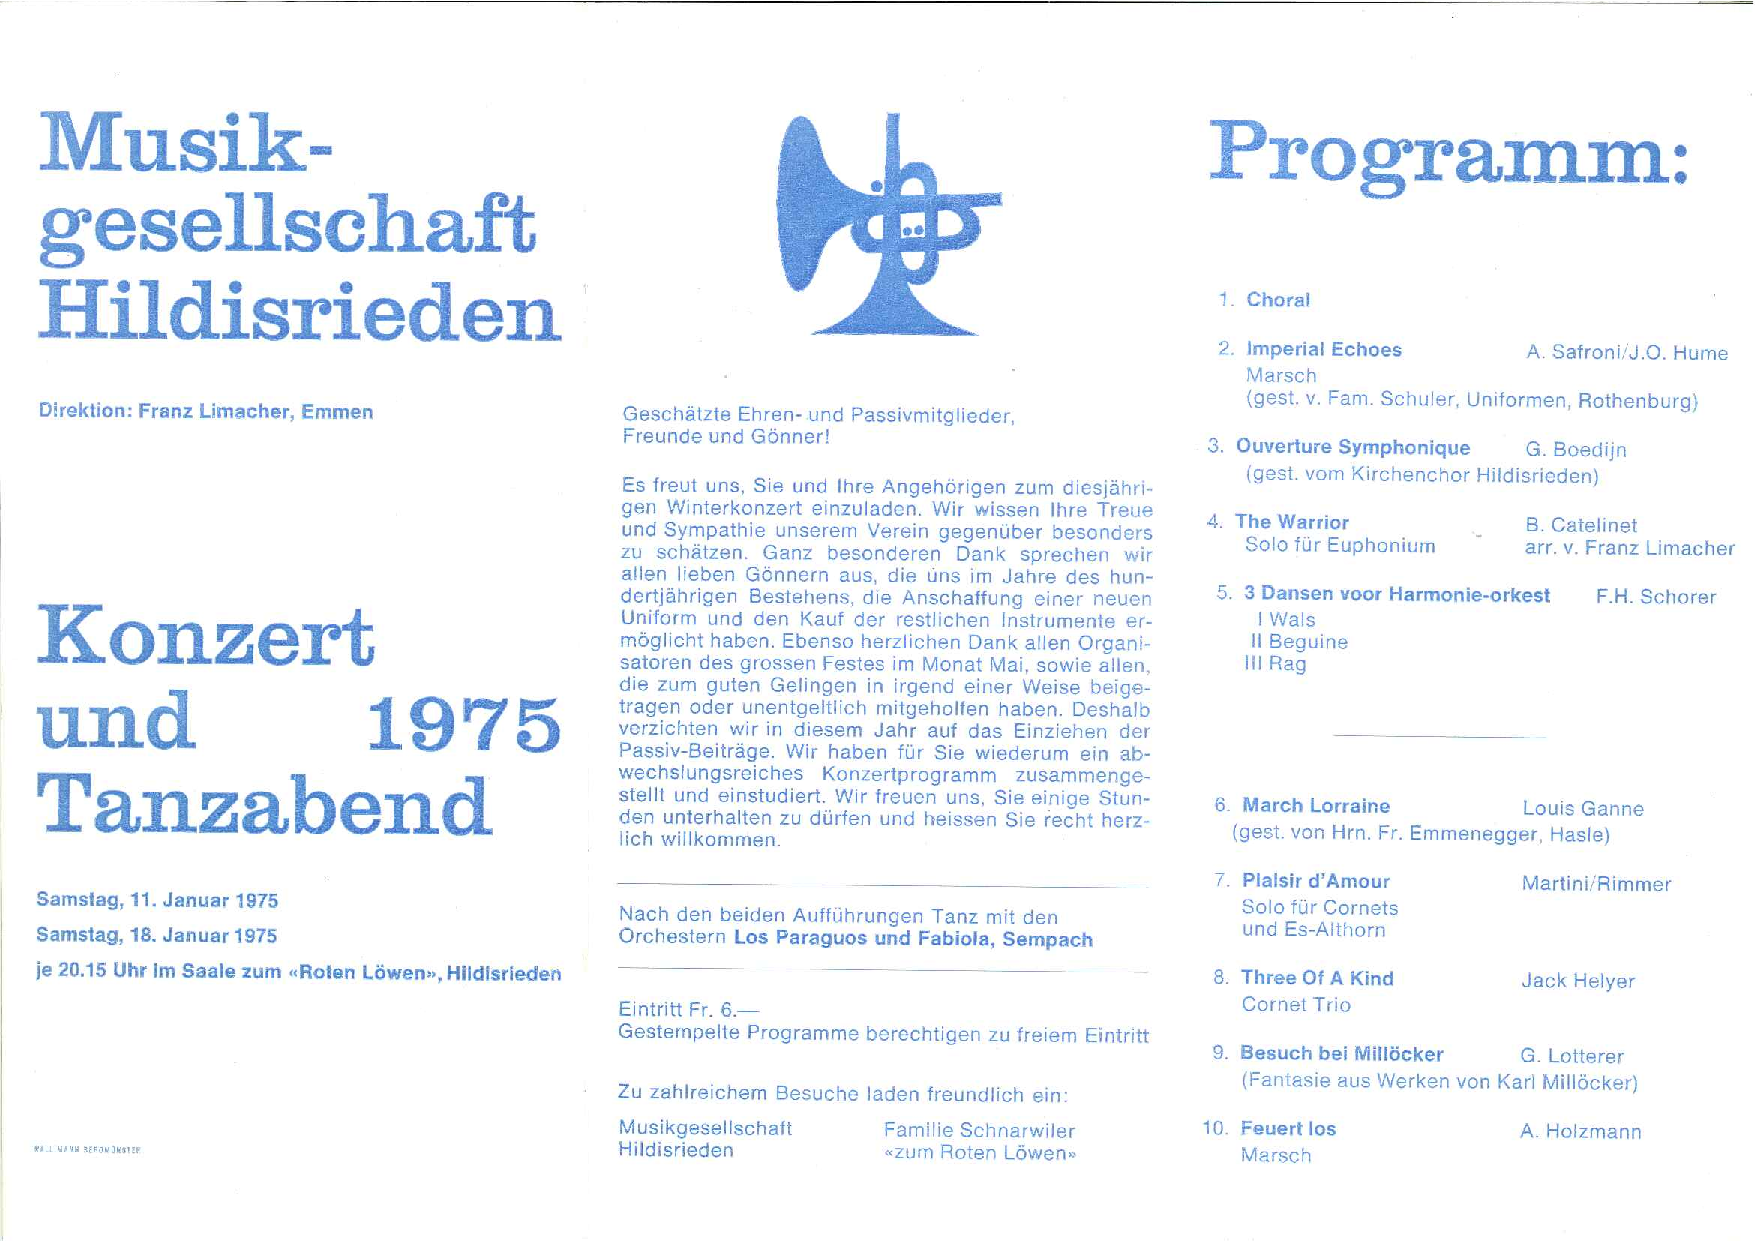
\includegraphics[scale=0.7]{./chap/1975/1975.pdf}
\end{figure}
\begin{multicols}{2}

    % \subsection{Jahresbericht}

    \begin{itemize}

        \item[]3. Jan.\\
        Um 20 Uhr holen wir den Zunftmeister von 1974 Alois Gassmann
        bei seinem Hause ab. Dann geht es mit Fackeln und Marschmusik durchs Dorf in den Löwen.
        Nach den üblichen Traktanden wird mit grossem Applaus Gemeindepräsident
        Werner Troxler-Käppeli, Moos, zum neuen Zunftmeister erkoren.

        \item[]7. Jan.\\
        Wir beschliessen, in diesem Jahr auf den Musikhock im Kreuz am schmutzigen Donnerstag zu verzichten,
        weil die Fastnacht so kurz ist.

        \item[]11. und 18. Jan.\\
        An diesen Abenden bringen wir das Winterkonzert zu Gehör. Der Löwensaal ist jeweils sehr gut besetzt.

        \item[]16. Jan.\\
        Wir begeben uns nach Emmen, um im Pfarreisaal unser Konzert der Emmer Bevölkerung aufzuführen.
        Leider sind nur sehr wenig Zuhörer anwesend.

        \item[]4. Feb.\\
        Wir begleiten den Zunftmeister zum Schulbesuch. Mit Marschmusik geht es durchs Dorf auf den alten Schulhausplatz.
        Während der Orangenschlacht spielen wir einige Märsche.

        \item[]6. April\\
        Wegen starkem Schneefall kann der Einzug am Weissen Sonntag nicht abgehalten werden.

        \item[]15. April\\
        Wir beschliessen, den Lohn von Direktor Franz Limacher von 3000 auf 3400 Fr. zu erhöhen.

        \item[]11. Mai\\
        Muttertagständchen. Löwenwirt J. Schnarwiler zahlt danach noch ein Bier.

        \item[]24. Mai\\
        Zur Expertise für das kommende kantonale Musikfest in Sempach laden wir André Winkler zur
        Probe in die Turnhalle ein. Mit träfen Worten erläutert er uns die schwachen Stellen der
        "`nostalgischen Ouvertüre"' und der "`Ouverture Symphonique"'.

        \item[]13. und 14. Juni\\
        Im Löwen und in der Kirche bringen die Musikgesellschaft Römerswil und die Musikgesellschaft Hildisrieden
        abwechslungsweise ihre Wettstücke für das kant. Musikfest in Sempach zur Aufführung.

        \item[]22. Juni\\
        Kant. Musikfest in Sempach.

        Wir spielen in der Festhalle das Aufgabestück "`Nostalgische Ouverture"',
        wir bekommen von der Jury schöne 153 von 180 Punkten. In der Kirche spielen wir das Selbstwahlstück
        "'Ouverture Symphonique"'. Hier erhalten wir 160 Punkte.
        Mit der Totalpunktzahl von 313 erreichen wir den 5. Rang in der 2. Stärkeklasse.

        Von der Marschmusikjury erhalten wir am Nachmittag leider nur 29 Punkte.
        Am Abend wird die MGH von der Götschizunft und der Dorfbevölkerung empfangen.
        Im Löwen werden wir von der Trachtengruppe und dem Kirchenchor unterhalten.

        \item[]20. Juli\\
        Wir können das Waldfest bei schönem Wetter durchführen. Die Tanzmusik "`The King Drivers"'
        bringt die Gäste zum Tanzen.



    \end{itemize}

\end{multicols}



\end{document}